\documentclass[11pt]{article}

%%%%%%%%%%%%%%%%%%%%%%%%%%%%%%%%%%%%%%%%%%%%%%%%%%%%%%%%%%%%%%%
%                      Customize Header                       %
%%%%%%%%%%%%%%%%%%%%%%%%%%%%%%%%%%%%%%%%%%%%%%%%%%%%%%%%%%%%%%%

\newcommand{\assessmentTitle}{
CheckIt Assessment
}
\newcommand{\assessmentVersion}{
Version 1770938997663
}
\newcommand{\assessmentInstructions}{
Do not use any unapproved aids while taking this assessment.
Read each question carefully and be sure to show all work
in the space provided.
}

%%%%%%%%%%%%%%%%%%%%%%%%%%%%%%%%%%%%%%%%%%%%%%%%%%%%%%%%%%%%%%%
%%%%%%%%%%%%%%%%%%%%%%%%%%%%%%%%%%%%%%%%%%%%%%%%%%%%%%%%%%%%%%%



\usepackage{amsfonts,amssymb,amsmath,amsthm}
\setcounter{MaxMatrixCols}{50}
\usepackage{hyperref}
\let\oldhref\href\renewcommand{\href}[2]{\oldhref{#1}{#2}\footnote{\url{#1}}}
\usepackage[margin=1in,tmargin=2in,headheight=84pt]{geometry}
\usepackage{enumerate}
\usepackage{graphicx}
\usepackage{fancyhdr}
\usepackage{lastpage}
\pagestyle{fancy}
\fancyhf{}
\rhead{Name: \underline{\hspace{2.5in}}\\ID: \underline{\hspace{2.5in}}

\vspace{2.5em}}
\chead{\vspace{2.5em}

\fbox{\fbox{\parbox{6in}{\centering\assessmentInstructions}}}}
\lhead{\assessmentTitle \hspace{2em} \assessmentVersion

\vspace{2.5em}}
\rfoot{Page \thepage\ of \pageref{LastPage}}
\setlength{\headheight}{80pt}
\renewcommand{\headrulewidth}{0pt}


\begin{document}

\begin{enumerate}

% 

\item %%%%% SpaTeXt Commands %%%%%
\providecommand{\stxKnowl}{}\renewcommand{\stxKnowl}[1]{#1}
\providecommand{\stxOuttro}{}\renewcommand{\stxOuttro}[1]{#1}
\providecommand{\stxTitle}{}\renewcommand{\stxTitle}[1]{#1}
% Comment next line to show outtros
\renewcommand{\stxOuttro}[1]{}
%%%%%%%%%%%%%%%%%%%%%%%%%%%%
\stxKnowl{
 Simplify: \(2 - 5( 20 - |12 - 6^2| )\) 

\stxOuttro{
SOLUTION

 \(2 - 5( 20 - |12 - 6^2| )\) 

 \(= 2 - 5( 20 - |12 - 36| )\) 

 \(= 2 - 5( 20 - |-24| )\) 

 \(= 2 - 5( 20 - 24 )\) 

 \(= 2 - 5( -4 )\) 

 \(= 2 - ( -20 )\) 

 \(= \boxed{ 22 }\) 

}
}

\newpage

% 

\item %%%%% SpaTeXt Commands %%%%%
\providecommand{\stxKnowl}{}\renewcommand{\stxKnowl}[1]{#1}
\providecommand{\stxOuttro}{}\renewcommand{\stxOuttro}[1]{#1}
\providecommand{\stxTitle}{}\renewcommand{\stxTitle}[1]{#1}
% Comment next line to show outtros
\renewcommand{\stxOuttro}[1]{}
%%%%%%%%%%%%%%%%%%%%%%%%%%%%
\stxKnowl{
 Simplify the radical expression completely: 

 \(4 \sqrt[3]{ -189 }\) 

\stxOuttro{
SOLUTION

 \(4 \sqrt[3]{ -189 }\) 

 \(= 4 \cdot \sqrt[3]{ -27 \cdot 7 }\) 

 \(= 4 \cdot (-3) \sqrt[3]{ 7 }\) 

 \(= \boxed{ -12 \sqrt[3]{ 7 } }\) 

}
}

\newpage

% 

\item %%%%% SpaTeXt Commands %%%%%
\providecommand{\stxKnowl}{}\renewcommand{\stxKnowl}[1]{#1}
\providecommand{\stxOuttro}{}\renewcommand{\stxOuttro}[1]{#1}
\providecommand{\stxTitle}{}\renewcommand{\stxTitle}[1]{#1}
% Comment next line to show outtros
\renewcommand{\stxOuttro}[1]{}
%%%%%%%%%%%%%%%%%%%%%%%%%%%%
\stxKnowl{
 Simplify: \(\displaystyle \left( \frac{ -3 a^{0} b^{0} c^{1} }{ a^{-2} b^{3} c^{2} } \right)^{ -3 }\) 

\stxOuttro{
SOLUTION

 \(\displaystyle \left( \frac{ -3 a^{0} b^{0} c^{1} }{ a^{-2} b^{3} c^{2} } \right)^{ -3 }\) 

 \(= \left( -3 a^{2} b^{-3} c^{-1} \right)^{-3}\) 

 \(= (-3)^{-3} a^{-6} b^{9} c^{3}\) 

 \(= \boxed{ - \frac{b^{9}c^{3}}{27a^{6}} }\) 

}
}

\newpage

% 

\item %%%%% SpaTeXt Commands %%%%%
\providecommand{\stxKnowl}{}\renewcommand{\stxKnowl}[1]{#1}
\providecommand{\stxOuttro}{}\renewcommand{\stxOuttro}[1]{#1}
\providecommand{\stxTitle}{}\renewcommand{\stxTitle}[1]{#1}
% Comment next line to show outtros
\renewcommand{\stxOuttro}[1]{}
%%%%%%%%%%%%%%%%%%%%%%%%%%%%
\stxKnowl{
 Simplify: \((4 \, x^{2} - 8 \, x - 3) - (-2 \, x^{2} + x + 9)\) 

\stxOuttro{
SOLUTION

 \((4 \, x^{2} - 8 \, x - 3) - (-2 \, x^{2} + x + 9)\) 

 \(= 4x^2-8x-3+2x^2-x-9\) 

 \(= 4x^2+2x^2-8x-x-3-9\) 

 \(= \boxed{ 6 \, x^{2} - 9 \, x - 12 }\) 

}
}

\newpage

% 

\item %%%%% SpaTeXt Commands %%%%%
\providecommand{\stxKnowl}{}\renewcommand{\stxKnowl}[1]{#1}
\providecommand{\stxOuttro}{}\renewcommand{\stxOuttro}[1]{#1}
\providecommand{\stxTitle}{}\renewcommand{\stxTitle}[1]{#1}
% Comment next line to show outtros
\renewcommand{\stxOuttro}[1]{}
%%%%%%%%%%%%%%%%%%%%%%%%%%%%
\stxKnowl{
 Simplify: \((2u - 2v)(4u^2 + 4uv + 4v^2)\) 

\stxOuttro{
SOLUTION

 \((2u - 2v)(4u^2 + 4uv + 4v^2)\) 

 \(= 2u(4u^2 + 4uv + 4v^2) - 2v(4u^2 + 4uv + 4v^2)\) 

 \(= 8u^3 + 8u^2v + 8uv^2 - 8u^2v - 8uv^2 - 8v^3\) 

 \(= \boxed{ 8u^3 - 8v^3 }\) 

}
}

\newpage

% 

\item %%%%% SpaTeXt Commands %%%%%
\providecommand{\stxKnowl}{}\renewcommand{\stxKnowl}[1]{#1}
\providecommand{\stxOuttro}{}\renewcommand{\stxOuttro}[1]{#1}
\providecommand{\stxTitle}{}\renewcommand{\stxTitle}[1]{#1}
% Comment next line to show outtros
\renewcommand{\stxOuttro}[1]{}
%%%%%%%%%%%%%%%%%%%%%%%%%%%%
\stxKnowl{
 Simplify: \(\displaystyle \frac{ 3 \, x^{4} + 10 \, x^{3} + 23 \, x^{2} + 23 \, x - 4 }{ 3 \, x + 4 }\) 

\stxOuttro{
SOLUTION

 \(\begin{array}{r} x^{3} + 2 \, x^{2} + 5 \, x + 1 \\ 3 \, x + 4 \overline{ ) 3 \, x^{4} + 10 \, x^{3} + 23 \, x^{2} + 23 \, x - 4 } \\ \underline{ -( 3 \, x^{4} + 4 \, x^{3} ) } \\\\ 6 \, x^{3} + 23 \, x^{2} + 23 \, x - 4 \\ \underline{ -( 6 \, x^{3} + 8 \, x^{2} ) } \\\\ 15 \, x^{2} + 23 \, x - 4 \\ \underline{ -( 15 \, x^{2} + 20 \, x ) } \\\\ 3 \, x - 4 \\ \underline{ -( 3 \, x + 4 ) } \\\\ -8 \end{array}\) 

 \(= \boxed{ x^{3} + 2 \, x^{2} + 5 \, x + 1 - \frac{8}{3 \, x + 4} }\) 

}
}

\newpage

% 

\item %%%%% SpaTeXt Commands %%%%%
\providecommand{\stxKnowl}{}\renewcommand{\stxKnowl}[1]{#1}
\providecommand{\stxOuttro}{}\renewcommand{\stxOuttro}[1]{#1}
\providecommand{\stxTitle}{}\renewcommand{\stxTitle}[1]{#1}
% Comment next line to show outtros
\renewcommand{\stxOuttro}[1]{}
%%%%%%%%%%%%%%%%%%%%%%%%%%%%
\stxKnowl{
 Solve: \(8 - 3(2x - 6) = 2(2x - 2)\) 

\stxOuttro{
SOLUTION

 \(8 - 3(2x - 6) = 2(2x - 2)\) 

 \(8 - 6x + 18 = 4x - 4\) 

 \(26 - 6x = 4x - 4\) 

 \(26 = 10x - 4\) 

 \(30 = 10x\) 

 \(\boxed{ x = 3 }\) 

}
}

\newpage

% 

\item %%%%% SpaTeXt Commands %%%%%
\providecommand{\stxKnowl}{}\renewcommand{\stxKnowl}[1]{#1}
\providecommand{\stxOuttro}{}\renewcommand{\stxOuttro}[1]{#1}
\providecommand{\stxTitle}{}\renewcommand{\stxTitle}[1]{#1}
% Comment next line to show outtros
\renewcommand{\stxOuttro}[1]{}
%%%%%%%%%%%%%%%%%%%%%%%%%%%%
\stxKnowl{
 Solve: \(\displaystyle \frac{1}{2}x - \frac{5}{16} = 2\) 

\stxOuttro{
SOLUTION

 \(\displaystyle \frac{1}{2}x - \frac{5}{16} = 2\) 

 \(16 \left( \frac{1}{2}x - \frac{5}{16} = 2 \right)\) 

 \(8x - 5 = 32\) 

 \(8x = 37\) 

 \(x = \frac{37}{8}\) 

 \(\boxed{ x = \frac{37}{8} }\) 

}
}

\newpage

% 

\item %%%%% SpaTeXt Commands %%%%%
\providecommand{\stxKnowl}{}\renewcommand{\stxKnowl}[1]{#1}
\providecommand{\stxOuttro}{}\renewcommand{\stxOuttro}[1]{#1}
\providecommand{\stxTitle}{}\renewcommand{\stxTitle}[1]{#1}
% Comment next line to show outtros
\renewcommand{\stxOuttro}[1]{}
%%%%%%%%%%%%%%%%%%%%%%%%%%%%
\stxKnowl{
 Solve for \(x\): \(rx + sy = t\) 

\stxOuttro{
SOLUTION

 \(rx + sy = t\) 

 \(rx = t - sy\) 

 \(\boxed{ x = \frac{t - sy}{r} }\) 

}
}

\newpage

% 

\item %%%%% SpaTeXt Commands %%%%%
\providecommand{\stxKnowl}{}\renewcommand{\stxKnowl}[1]{#1}
\providecommand{\stxOuttro}{}\renewcommand{\stxOuttro}[1]{#1}
\providecommand{\stxTitle}{}\renewcommand{\stxTitle}[1]{#1}
% Comment next line to show outtros
\renewcommand{\stxOuttro}[1]{}
%%%%%%%%%%%%%%%%%%%%%%%%%%%%
\stxKnowl{
 A rental car costs $\(30.00\) per day plus $\(0.25\) per mile driven. If Dana has $\(89.75\) for a one-day rental, how many miles can they drive? 

\stxOuttro{
SOLUTION

 \(89.75 - 30.00 = 59.75\) 

 \(\frac{59.75}{0.25} = 239\) 

 \(\boxed{ 239 \text{ miles} }\) 

}
}

\newpage

% 

\item %%%%% SpaTeXt Commands %%%%%
\providecommand{\stxKnowl}{}\renewcommand{\stxKnowl}[1]{#1}
\providecommand{\stxOuttro}{}\renewcommand{\stxOuttro}[1]{#1}
\providecommand{\stxTitle}{}\renewcommand{\stxTitle}[1]{#1}
% Comment next line to show outtros
\renewcommand{\stxOuttro}[1]{}
%%%%%%%%%%%%%%%%%%%%%%%%%%%%
\stxKnowl{
 Graph and identify the slope and intercepts of the function: \(f(x) = -\frac{6}{5}x - 6\) 

 \begin{tikzpicture}[scale=0.4] \draw[help lines, color=gray!50] (-10,-10) grid (10,10); \draw[<->, thick] (-10.5,0)--(10.5,0) node[right]{$x$}; \draw[<->, thick] (0,-10.5)--(0,10.5) node[above]{$y$}; \end{tikzpicture} 

\stxOuttro{
SOLUTION

 \(\text{Slope: } m = -\frac{6}{5}\) 

 \(\text{y-intercept: } (0, -6)\) 

 \(\text{x-intercept: } (-5, 0)\) 

 \begin{tikzpicture}[scale=0.4] \draw[help lines, color=gray!50] (-10,-10) grid (10,10); \draw[<->, thick] (-10.5,0)--(10.5,0) node[right]{$x$}; \draw[<->, thick] (0,-10.5)--(0,10.5) node[above]{$y$}; \begin{scope} \clip (-10,-10) rectangle (10,10); \draw[<->, ultra thick, blue, domain=-11:11, samples=2] plot (\x, {-1.2*\x + -6.0}); \end{scope} \fill[red] (-5,0) circle (0.3); \fill[red] (0,-6) circle (0.3); \end{tikzpicture} 

}
}

\newpage

% 

\item %%%%% SpaTeXt Commands %%%%%
\providecommand{\stxKnowl}{}\renewcommand{\stxKnowl}[1]{#1}
\providecommand{\stxOuttro}{}\renewcommand{\stxOuttro}[1]{#1}
\providecommand{\stxTitle}{}\renewcommand{\stxTitle}[1]{#1}
% Comment next line to show outtros
\renewcommand{\stxOuttro}[1]{}
%%%%%%%%%%%%%%%%%%%%%%%%%%%%
\stxKnowl{
 Given \(g(x) = x^2 - 9x + 3\), find each of the following. 

\begin{enumerate}
\item
\stxKnowl{
 \(g(-1)\) 

\stxOuttro{
 \(g(-1) = (-1)^2 - 9(-1) + 3\) 

 \(= 1 + 9 + 3\) 

 \(= \boxed{ 13 }\) 

}
}

\item
\stxKnowl{
 \(g(0)\) 

\stxOuttro{
 \(g(0) = (0)^2 - 9(0) + 3\) 

 \(= \boxed{ 3 }\) 

}
}

\item
\stxKnowl{
 \(g(x+h)\) 

\stxOuttro{
 \(g(x+h) = (x+h)^2 - 9(x+h) + 3\) 

 \(= \boxed{ x^2 + 2xh + h^2 - 9x - 9h + 3 }\) 

}
}

\end{enumerate}
}

\newpage

% 

\item %%%%% SpaTeXt Commands %%%%%
\providecommand{\stxKnowl}{}\renewcommand{\stxKnowl}[1]{#1}
\providecommand{\stxOuttro}{}\renewcommand{\stxOuttro}[1]{#1}
\providecommand{\stxTitle}{}\renewcommand{\stxTitle}[1]{#1}
% Comment next line to show outtros
\renewcommand{\stxOuttro}[1]{}
%%%%%%%%%%%%%%%%%%%%%%%%%%%%
\stxKnowl{
 For each graph below, determine whether it represents a function and identify the domain and range. 

\begin{enumerate}
\item
\stxKnowl{
 \begin{tikzpicture}[scale=0.35] \draw[step=2cm, gray!40, very thin] (-10,-10) grid (10,10); \draw[thick, <->] (-10.5,0) -- (10.5,0) node[right] {$x$}; \draw[thick, <->] (0,-10.5) -- (0,10.5) node[above] {$y$}; \foreach \x in {-10,-8,...,10} \draw (\x, 0.1) -- (\x, -0.1) node[below] {\tiny $\x$}; \foreach \y in {-10,-8,...,10} \draw (0.1, \y) -- (-0.1, \y) node[left] {\tiny $\y$}; \draw[ultra thick, blue, <->, domain=-9.32455532033676:3.324555320336759, samples=100] plot (\x, {0.250000000000000*(\x - -3)^2 + 0}); \end{tikzpicture} 

\stxOuttro{
Solution

\begin{itemize}
\item
Domain: \((-\infty, \infty)\)

\item
Range: \([0, \infty)\)

\item
Function

\end{itemize}
}
}

\item
\stxKnowl{
 \begin{tikzpicture}[scale=0.35] \draw[step=2cm, gray!40, very thin] (-10,-10) grid (10,10); \draw[thick, <->] (-10.5,0) -- (10.5,0) node[right] {$x$}; \draw[thick, <->] (0,-10.5) -- (0,10.5) node[above] {$y$}; \foreach \x in {-10,-8,...,10} \draw (\x, 0.1) -- (\x, -0.1) node[below] {\tiny $\x$}; \foreach \y in {-10,-8,...,10} \draw (0.1, \y) -- (-0.1, \y) node[left] {\tiny $\y$}; \draw[ultra thick, blue, <->, domain=-2.6568542494923806:8.65685424949238, samples=100] plot ({0.250000000000000*(\x - 3)^2 + 2}, \x); \end{tikzpicture} 

\stxOuttro{
Solution

\begin{itemize}
\item
Domain: \([2, \infty)\)

\item
Range: \((-\infty, \infty)\)

\item
Not a function

\end{itemize}
}
}

\end{enumerate}
}

\newpage

% 

\item %%%%% SpaTeXt Commands %%%%%
\providecommand{\stxKnowl}{}\renewcommand{\stxKnowl}[1]{#1}
\providecommand{\stxOuttro}{}\renewcommand{\stxOuttro}[1]{#1}
\providecommand{\stxTitle}{}\renewcommand{\stxTitle}[1]{#1}
% Comment next line to show outtros
\renewcommand{\stxOuttro}[1]{}
%%%%%%%%%%%%%%%%%%%%%%%%%%%%
\stxKnowl{
 Given the graph of the function \(f\) below, find each of the following. 

 \begin{tikzpicture}[scale=0.35] \draw[step=1cm, gray!40, very thin] (-10,-10) grid (10,10); \draw[thick, <->] (-10.5,0) -- (10.5,0) node[right] {$x$}; \draw[thick, <->] (0,-10.5) -- (0,10.5) node[above] {$y$}; \foreach \x in {-10,-8,...,10} \draw (\x, 0.1) -- (\x, -0.1) node[below] {\tiny $\x$}; \foreach \y in {-10,-8,...,10} \draw (0.1, \y) -- (-0.1, \y) node[left] {\tiny $\y$}; \draw[ultra thick, blue, <->, domain=-8.32455532033676:4.324555320336759, samples=100] plot (\x, {0.250000000000000*(\x - -2)^2 + 0}); \end{tikzpicture} 

\begin{itemize}
\item
(a) \(f(0)\)

\item
(b) \(f(-8)\)

\item
(c) \(f(-6)\)

\item
(d) Find \(x\) where \(f(x) = 0\)

\end{itemize}
\stxOuttro{
Solution

\begin{itemize}
\item
(a) \(1\)

\item
(b) \(9\)

\item
(c) \(4\)

\item
(d) \(x = -2\)

\end{itemize}
}
}

\newpage

% 

\item %%%%% SpaTeXt Commands %%%%%
\providecommand{\stxKnowl}{}\renewcommand{\stxKnowl}[1]{#1}
\providecommand{\stxOuttro}{}\renewcommand{\stxOuttro}[1]{#1}
\providecommand{\stxTitle}{}\renewcommand{\stxTitle}[1]{#1}
% Comment next line to show outtros
\renewcommand{\stxOuttro}[1]{}
%%%%%%%%%%%%%%%%%%%%%%%%%%%%
\stxKnowl{
 Find the equation of the line parallel to \(6x - 6y = -8\) and passing through \((-2, -6)\). 

\stxOuttro{
Solution

Slope:

 \(6x - 6y = -8\) 

 \(-6y = -6x + -8\) 

 \(y = 1x + \frac{4}{3}\) 

 \(m = 1\) 

Y-intercept:

 \(y = mx + b\) 

 \(-6 = 1(-2) + b\) 

 \(-6 = -2 + b\) 

 \(b = -4\) 

 \(\boxed{ y = 1x - 4 }\) 

}
}

\newpage

% 

\item %%%%% SpaTeXt Commands %%%%%
\providecommand{\stxKnowl}{}\renewcommand{\stxKnowl}[1]{#1}
\providecommand{\stxOuttro}{}\renewcommand{\stxOuttro}[1]{#1}
\providecommand{\stxTitle}{}\renewcommand{\stxTitle}[1]{#1}
% Comment next line to show outtros
\renewcommand{\stxOuttro}[1]{}
%%%%%%%%%%%%%%%%%%%%%%%%%%%%
\stxKnowl{
 A particular search engine assigns a ranking to a webpage based on the number of links that direct users to the webpage. The ranking of a webpage is given by the function below, where \(n\) represents the number of links that direct users to it. How many links will be needed to obtain a page ranking of 10? 

 \(R(n) = \frac{1}{21}n + 5\) 

\stxOuttro{
Solution

 \(10 = \frac{1}{21}n + 5\) 

 \(5 = \frac{1}{21}n\) 

 \(105 = n\) 

 \(\boxed{ 105 \text{ links} }\) 

}
}

\newpage

% 

\item %%%%% SpaTeXt Commands %%%%%
\providecommand{\stxKnowl}{}\renewcommand{\stxKnowl}[1]{#1}
\providecommand{\stxOuttro}{}\renewcommand{\stxOuttro}[1]{#1}
\providecommand{\stxTitle}{}\renewcommand{\stxTitle}[1]{#1}
% Comment next line to show outtros
\renewcommand{\stxOuttro}[1]{}
%%%%%%%%%%%%%%%%%%%%%%%%%%%%
\stxKnowl{
 Solve the system of equations. 

 \(\begin{cases} x - y = 4 \\ x + y = -12 \end{cases}\) 

\stxOuttro{
Solution

 \(x - y = 4 \to x = y + 4\) 

Substitute:

 \((y + 4) + y = -12\) 

 \(2y + 4 = -12\) 

 \(2y = -16\) 

 \(y = -8\) 

Back-substitute:

 \(x = -8 + 4\) 

 \(x = -4\) 

 \(\boxed{ (-4, -8) }\) 

}
}

\newpage

% 

\end{enumerate}

\end{document}